\section{Phase-Rejoining Residual \SMPCC{} Method}
\label{sec:method}

\subsection{Problem, Core Idea, and Scope}

We consider a differential-drive mobile base carrying an open liquid along a geometrically feasible path that is fixed before motion.
An offline anti-slosh sequence can coordinate an initial excitation with a later cancellation, slowdown, and settling tail.
A conventional online tracker may nevertheless alter the speed or turn rate to reduce an immediate path error and thereby invalidate the remaining cancellation.
The central design rule is therefore:
\emph{an online residual may correct tracking, but it is admitted only if the state predicted after the real execution delays remains eligible to rejoin the phase-indexed offline tail.}

Figure~\ref{fig:core_architecture} shows the resulting offline--online structure.
The offline layer owns the complete nominal motion and tail.
The online layer aligns the available state to the expected publication epoch, selects one nearby monotone artifact phase, and optimizes a bounded residual through the unequal linear and angular execution delays.
At the terminal prediction step, a 9-D robot--liquid empirical gate and a compatibility set for the pending execution state must both hold.
This is a hard admission test, not an additional soft slosh penalty.

\begin{figure*}[t]
  \centering
  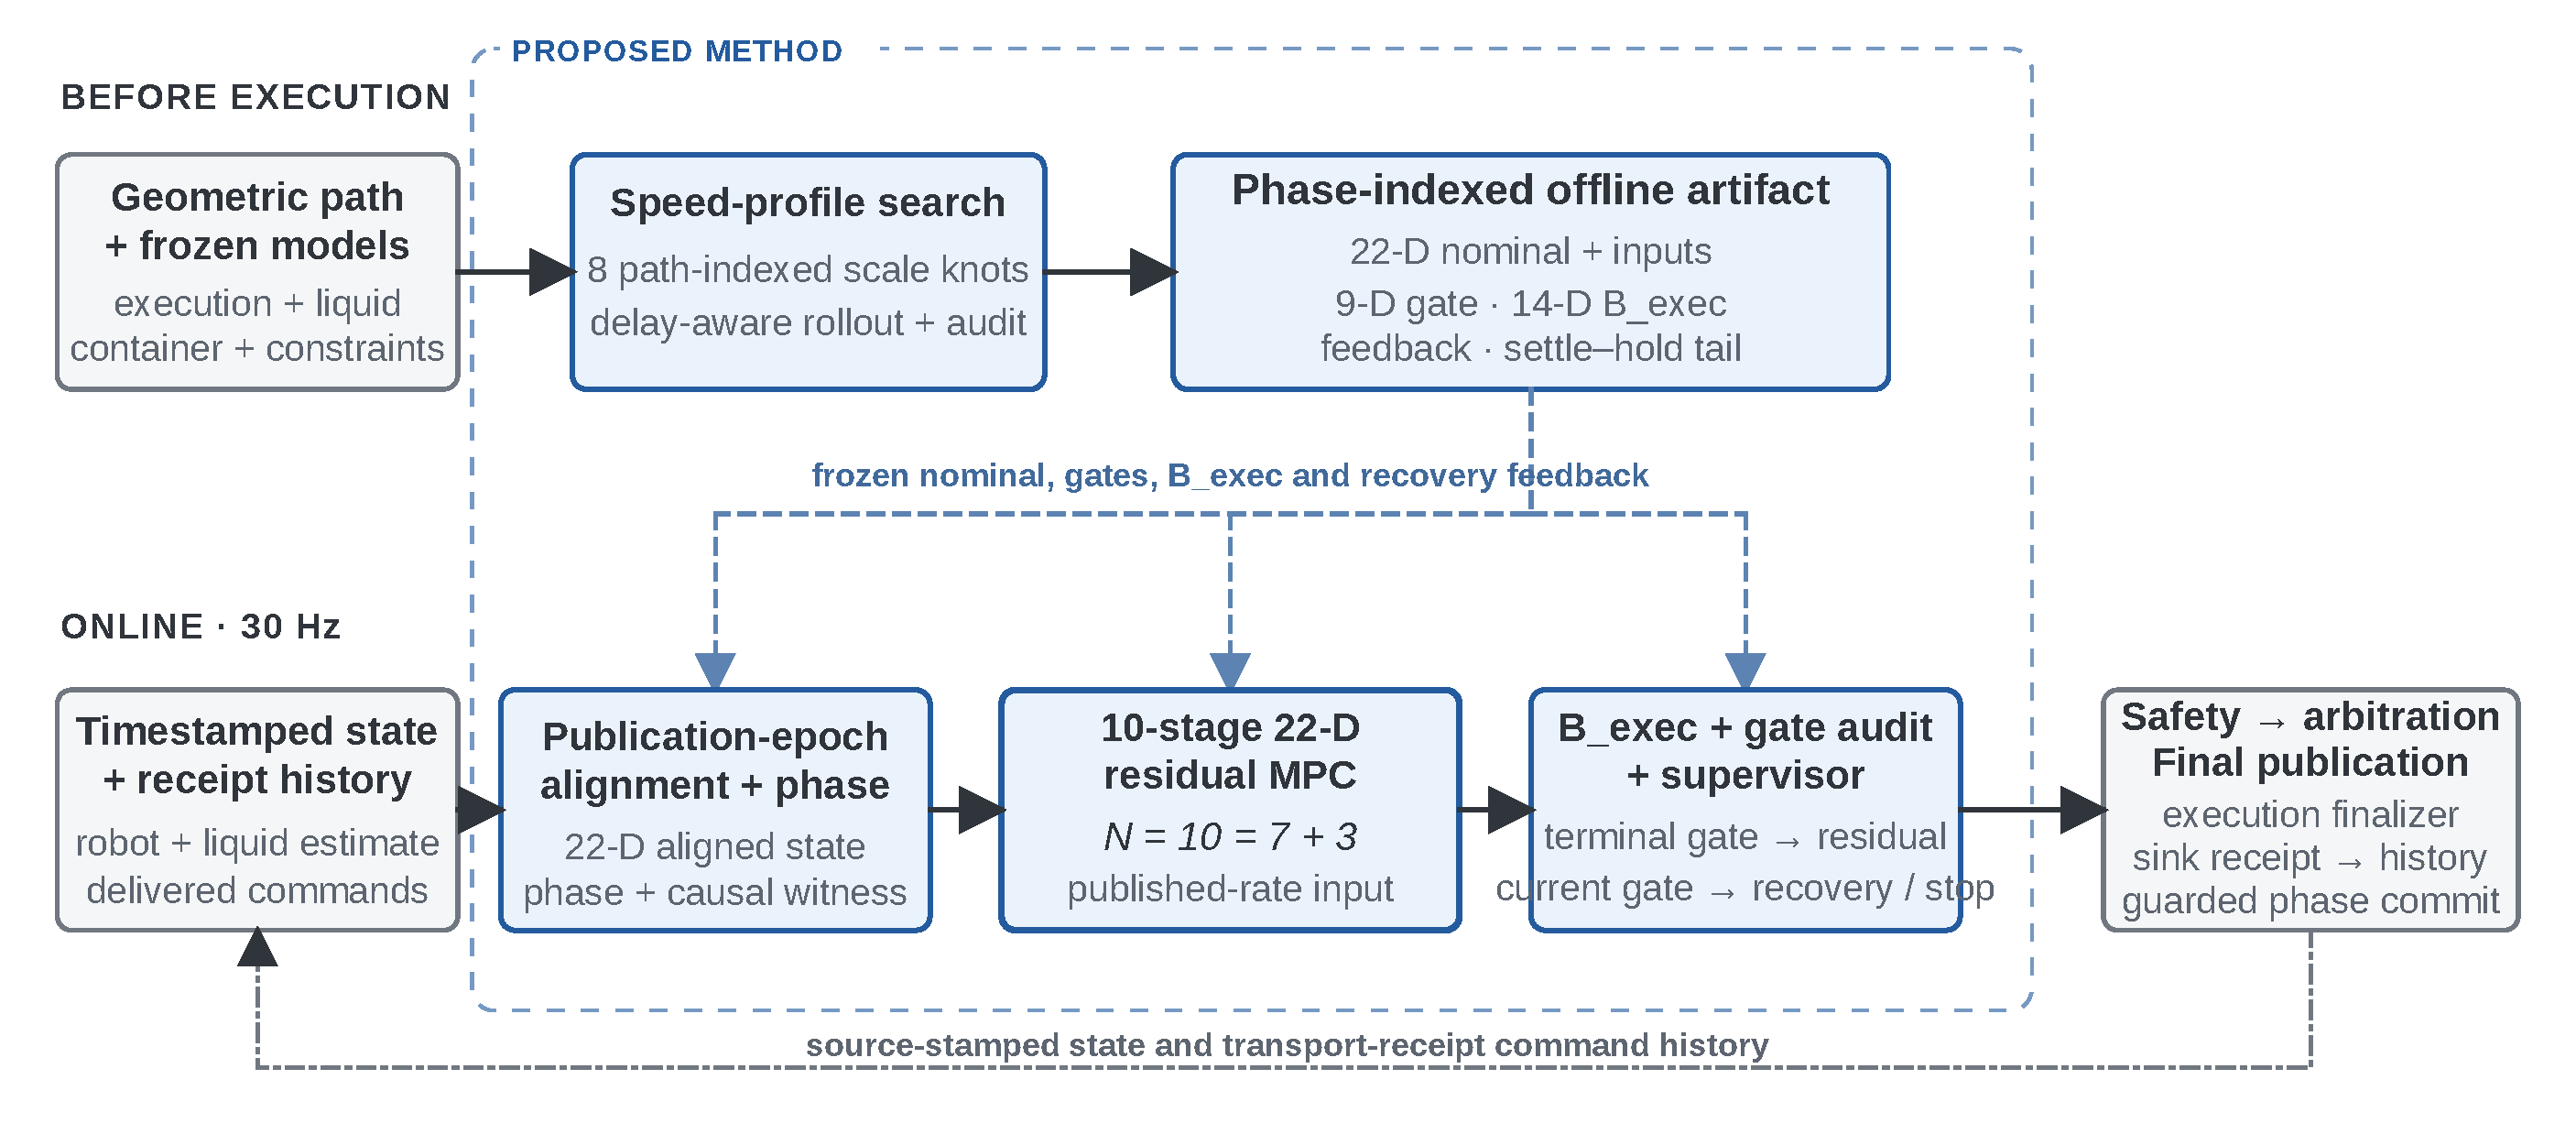
\includegraphics[width=\textwidth]{figures/phase_rejoining_framework_paper.pdf}
  \caption{Overview of \PRSMPCC{}.
  Before execution, OfflineSloshOCP turns the fixed path and frozen execution--liquid models into a phase-indexed artifact with a complete motion--settle--hold tail.
  Online, the state estimate is aligned with the execution front and a nearby monotone phase, and only bounded residuals that pass the joint rejoin test are admitted.
  The supervisor selects residual, recovery, or stop before the common safety and publication chain; measured response and the final published-command history close the loop.}
  \label{fig:core_architecture}
\end{figure*}

The scope is deliberately narrow: a frozen path, a frozen container/model contract, an initially admitted liquid state, and small runtime deviations.
The method performs no online obstacle detection, collision-corridor optimization, homotopy search, or replanning.
An MBF path may be generated before a trial, but its point sequence, frame, and hash must then be frozen and a path-specific offline artifact regenerated.

\subsection{Shared Model and Offline Artifact}

\subsubsection{Robot--liquid and execution state}

Let $\bm p=[p_x,p_y]^\top$ and $\psi$ denote planar position and yaw, and let $v^r$ and $\omega^r$ denote realized linear and angular motion.
For a reference curve $\bm r(s)$ with tangent angle $\psi_r(s)$, the usual lag and contour errors are
\begin{equation}
  \begin{bmatrix}e_l\\e_c\end{bmatrix}
  =
  \begin{bmatrix}
    \cos\psi_r & \sin\psi_r\\
    -\sin\psi_r & \cos\psi_r
  \end{bmatrix}
  \left(\bm p-\bm r(s)\right).
  \label{eq:contour_lag_errors}
\end{equation}
The progress variable $s$ is retained only locally around the selected offline phase; it is not a free global time-scaling variable as in a conventional unconstrained virtual-progress formulation \cite{D19_Liniger2015,D20_Brito2019}.

The liquid model retains the first lateral mode in two orthogonal container axes,
\begin{equation}
  z^\ell=
  [\eta_x,\dot\eta_x,\eta_y,\dot\eta_y]^\top,
  \qquad
  \dot z^\ell=A_\ell z^\ell+B_\ell
  \begin{bmatrix}\dot v^r\\v^r\omega^r\end{bmatrix},
  \label{eq:liquid_model}
\end{equation}
where $A_\ell$ and $B_\ell$ are obtained from the frozen container and liquid parameters.
This low-order representation follows equivalent mechanical slosh models used for two-dimensional excitation \cite{A01_Leva2021,A02_Guagliumi2021}.
It is an internal prediction state, not a direct measurement of the true signed liquid phase.

We distinguish three state descriptions:
\begin{align}
  \chi &=[p_x,p_y,\psi,v^r,\omega^r,z^{\ell\top}]^\top\in\mathbb R^9,
  \label{eq:gate_state}\\
  X &=\operatorname{col}(p_x,p_y,\psi,v^c,s,\omega^c,z^\ell),
  \label{eq:base_ocp_state}\\
  X^{\mathrm{aug}}&=\operatorname{col}(X,b^v,b^\omega,x^a).
  \label{eq:augmented_state}
\end{align}
For phase selection and gate construction, yaw is never subtracted as an unwrapped Euclidean coordinate.
We use the common 9-D error operator
\begin{equation}
\begin{split}
  \mathcal E_\chi(\chi,\bar\chi)=\operatorname{col}\big(&
  \bm p-\bar{\bm p},
  \operatorname{wrap}_{(-\pi,\pi]}(\psi-\bar\psi),\\
  &v^r-\bar v^r,\ \omega^r-\bar\omega^r,\
  z^\ell-\bar z^\ell\big).
\end{split}
\label{eq:gate_error_operator}
\end{equation}
Here $v^c$ and $\omega^c$ are command-integrator states, $b^v$ and $b^\omega$ are the linear and angular command buffers, and $x^a=[v^r,\omega^r]^\top$ contains the realized actuator states.
The acceleration-level OCP input is
\begin{equation}
  q=[a,\alpha,v_s]^\top,
  \label{eq:ocp_input}
\end{equation}
with linear acceleration $a$, angular acceleration $\alpha$, and local progress rate $v_s$.
Within the horizon, $q_k$ first generates a raw solver command and its hypothetical publishable counterpart,
\begin{align}
  u_k^{\mathrm{sol}}
  &=\begin{bmatrix}v_k^c+a_k\Delta t\\
                     \omega_k^c+\alpha_k\Delta t\end{bmatrix},
  \label{eq:solver_command_map}\\
  u_k^{\mathrm{pred}}
  &=\Pi_{\mathrm{cmd}}(u_k^{\mathrm{sol}},b_k^v,b_k^\omega),
  \label{eq:predicted_publishable_command}
\end{align}
where $\Pi_{\mathrm{cmd}}$ applies the frozen speed, acceleration, and rate limits modeled by the OCP.
It does not predict an independent safety override.
The command and local-progress states then satisfy
\begin{equation}
  \begin{bmatrix}v_{k+1}^c\\\omega_{k+1}^c\end{bmatrix}
  =u_k^{\mathrm{pred}},
  \qquad
  s_{k+1}=s_k+\Delta t\,v_{s,k}.
  \label{eq:command_progress_update}
\end{equation}

For channel $r\in\{v,\omega\}$, write
\begin{equation}
  m_r=\left\lfloor\frac{d_r}{\Delta t}\right\rfloor,
  \qquad
  \lambda_r=\frac{d_r}{\Delta t}-m_r.
  \label{eq:fractional_delay}
\end{equation}
The predicted FIFO shift and fractionally delayed setpoint are
\begin{align}
  b_{k+1}^{r,(0)}&=u_{r,k}^{\mathrm{pred}},
  &b_{k+1}^{r,(h+1)}&=b_k^{r,(h)},
  \label{eq:buffer_shift}\\
  \widetilde u_{r,k+1}
  &=(1-\lambda_r)b_{k+1}^{r,(m_r)}
    +\lambda_r b_{k+1}^{r,(m_r+1)},
  \label{eq:fractional_delay_output}
\end{align}
with $h=0{:}m_r$ and buffer entries $0{:}m_r+1$.
With identified gain $g_r$ and time constant $\tau_r$, the actuator update is
\begin{equation}
  x^a_{r,k+1}=\gamma_r x^a_{r,k}
  +(1-\gamma_r)g_r\widetilde u_{r,k+1},
  \qquad
  \gamma_r=e^{-\Delta t/\tau_r}.
  \label{eq:actuator_update}
\end{equation}
The realized $v^r=x_v^a$ and $\omega^r=x_\omega^a$ drive the base kinematics and the excitation in \eqref{eq:liquid_model}; in discrete time,
\begin{align}
  \bm p_{k+1}&=\bm p_k+\Delta t\,v_k^r
  [\cos\psi_k,\sin\psi_k]^\top,
  &\psi_{k+1}&=\psi_k+\Delta t\,\omega_k^r,
  \label{eq:realized_kinematics}\\
  a_{x,k}^r&=(v_{k+1}^r-v_k^r)/\Delta t,
  &a_{y,k}^r&=v_k^r\omega_k^r.
  \label{eq:realized_excitation}
\end{align}
Equations~\eqref{eq:solver_command_map}--\eqref{eq:realized_excitation}, the local progress update, and the discretized liquid model define
\begin{equation}
  X^{\mathrm{aug}}_{k+1}
  =F_{\mathrm{exec}\text{-}\ell}
  \left(X^{\mathrm{aug}}_k,u_k^{\mathrm{pred}},v_{s,k};\Theta\right),
  \label{eq:delay_augmented_dynamics}
\end{equation}
where $\Theta$ freezes the robot, liquid, unequal delay, buffer, and actuator parameters.

The superscript ``pred'' is confined to a hypothetical OCP rollout.
After supervision and all runtime overrides, the measured $u^{\mathrm{pub}}$ is the only command appended to the persistent buffers and used for delay identification; an unexecuted $u^{\mathrm{sol}}$ or $u^{\mathrm{pred}}$ is never written into command history.
At the next solve, the command-integrator state is reanchored to the latest final $u^{\mathrm{pub}}$ before constructing the rollout.

\subsubsection{Complete \OfflineSloshOCP{} artifact}

Input shaping and offline anti-slosh planning can exploit the complete motion rather than a truncated online preview \cite{A07_Singer1990,B03_Hamaguchi2004,B02_Hamaguchi2005,C01_Ferrari2026}.
For the frozen path and contract, \OfflineSloshOCP{} produces
\begin{equation}
  \bar{\mathcal A}=\left(
  \{\bar X_i^{\mathrm{aug}},\bar\chi_i,\bar t_i\}_{i=0}^{M},
  \{\bar q_i,\bar u_i^{\mathrm{pub}}\}_{i=0}^{M-1}
  \right).
  \label{eq:offline_artifact}
\end{equation}
Unlike a trajectory truncated at geometric arrival, $\bar{\mathcal A}$ includes motion, slowdown, liquid settling, and a verified zero-command hold.
The nominal buffer and actuator states are generated by passing the nominal published commands through the same execution model used online.
At the paper level, the offline problem is
\begin{subequations}
\label{eq:offline_ocp_contract}
\begin{align}
  \min_{\{\bar X_i^{\mathrm{aug}},\bar q_i\}}
  \quad &
  \bar J_{\mathrm{task}}+\bar J_{\mathrm{liquid}}
  +\bar J_{\mathrm{regularity}},
  \label{eq:offline_ocp_objective}\\
  \text{s.t.}\quad &
  \bar X_{i+1}^{\mathrm{aug}}
  =F_{\mathrm{exec}\text{-}\ell}
  (\bar X_i^{\mathrm{aug}},\bar u_i^{\mathrm{pred}},\bar v_{s,i};\Theta),
  \label{eq:offline_ocp_dynamics}\\
  &(\bar X_i^{\mathrm{aug}},\bar q_i)\in\mathcal Z,
  \label{eq:offline_ocp_constraints}\\
  &\bar u_i^{\mathrm{pub}}=(0,0),
  \quad i=M-N_h{:}M-1,
  \label{eq:offline_zero_hold}\\
  &\|\bar z_i^\ell\|\le\epsilon_{\mathrm{settle}},
  \quad i=M-N_h{:}M.
  \label{eq:offline_tail_constraint}
\end{align}
\end{subequations}
The three costs cover prescribed-path completion, modeled liquid response including the tail, and command regularity; their frozen definitions and weights belong to the supplementary release record.
$N_h$ and $\epsilon_{\mathrm{settle}}$ define the terminal zero hold before any formal artifact is built.

Each artifact phase $i$ additionally stores
\begin{equation}
  \left(
  \widehat{\mathcal R}^{\mathrm{emp}}_i,
  \mathcal B_i^{\mathrm{exec}},
  u_{\mathrm{rec}}(i)
  \right),
  \label{eq:phase_objects}
\end{equation}
where $\widehat{\mathcal R}^{\mathrm{emp}}_i$ is a 9-D empirical recovery gate, $\mathcal B_i^{\mathrm{exec}}$ is an execution-state compatibility set, and $u_{\mathrm{rec}}(i)$ is a phase-indexed stored action.
The artifact contract freezes the path and frame hashes, time grid, robot/execution/liquid models, container and fill range, constraints, complete tail, gate schema, and software version.
A change to any contracted object invalidates the artifact rather than silently reusing it.

The empirical objects are constructed from recovery rollouts around each phase.
A sample is labeled successful only when its execution state is compatible, the stored action is applied through the publication chain, the nominal tail is resumed, all constraints remain satisfied, and the preregistered settling rule is met.
On $D_{\mathrm{gate,fit}}$, a finite stored-action library and candidate values of $\rho_{r,i}$ and $\beta^{\mathrm{exec}}_{r,i}$ are evaluated by a frozen selection rule.
The target rule maximizes accepted coverage subject to minimum per-phase support and a preregistered upper confidence bound on the conditional false-safe fraction; a phase with no admissible candidate is marked unavailable.
The selected $u_{\mathrm{rec}}(i)$, radii, bounds, and unavailable phases are frozen before $D_{\mathrm{gate,test}}$ is opened.

\subsection{Execution-Front Alignment and Phase Rejoining}

\subsubsection{Expected publication epoch and unequal delays}

Let $t_s$ be the source timestamp of the latest admitted state and $t_c$ the start of the current computation.
With the frozen or online estimate $\widehat d_c$ of computation-to-publication delay, the prediction epoch is
\begin{equation}
  t=t_c+\widehat d_c,
  \label{eq:publication_epoch}
\end{equation}
not $t_c$.
The state is first propagated from $t_s$ to $t$ using timestamped published-command history and the known command held during computation.
The realized $d_c$ and error $d_c-\widehat d_c$ are logged and must be covered by the release validation or its disturbance bounds.

Let $d_v$ and $d_\omega$ be the command-to-motion delays identified from final publication timestamps, and let $\Delta t$ be the OCP grid.
Define
\begin{equation}
\begin{aligned}
  n_v&=\left\lceil\frac{d_v}{\Delta t}\right\rceil,
  &n_\omega&=\left\lceil\frac{d_\omega}{\Delta t}\right\rceil,\\
  n_f&=\max(n_v,n_\omega),
  &N_e&=n_f+N_\ell.
\end{aligned}
  \label{eq:execution_horizon}
\end{equation}
The first $n_f$ prediction steps represent causal propagation through the execution delays; the following $N_\ell$ steps form the short window in which both channels can respond.
The total source-to-terminal lead is
\begin{equation}
  T_{\mathrm{lead}}=(t-t_s)+N_e\Delta t.
  \label{eq:total_lead}
\end{equation}

The current candidate values are $d_v\simeq150$ ms, $d_\omega\simeq220$ ms, $\Delta t\simeq33.3$ ms, $n_f=7$, and $N_\ell=3$.
Thus, the grid-aligned common front occurs approximately $233.3$ ms after the expected publication epoch and the joint terminal test approximately $333.3$ ms after it.
The often quoted ``100-ms liquid window'' is only the interval after the common front, not the full prediction lead.

\paragraph{Current release blocker B0.}
The formulation above defines the target release.
Physical enforcement remains disabled in the current development revision because its history-only front predictor omits candidate-command dependence between the unequal delays: the new linear command can act for roughly $83$ ms before the common front.
It also mixes the physical front at about $0.22$ s with the grid index $7\Delta t\simeq0.2333$ s, an epoch error of about $13.3$ ms.
B0 must be resolved by the delay-augmented OCP in \eqref{eq:delay_augmented_dynamics}, or by a strictly equivalent decision-dependent condensed bridge, before the G0 release test and physical \texttt{enforce} mode.

\subsubsection{Neighboring monotone phase selection}

At control cycle $m$, let $\tau_m=t-t_0$ be elapsed artifact time at the expected publication epoch.
This clock advances with source/publication time even while a command is held and is reset only by admitting a new artifact execution; it is not an optimization variable.
The clock prior supplies $i_{\mathrm{clock},m}$ from $\tau_m$.
The admissible phase set is
\begin{equation}
  \mathcal J_m=\left\{j\in\mathbb Z:\
  \begin{aligned}
    i_{\mathrm{clock},m}-r_-&\le j\le i_{\mathrm{clock},m}+r_+,\\
    j&\ge j_{m-1},\\
    0&\le j\le M-N_e
  \end{aligned}
  \right\}.
  \label{eq:phase_candidates}
\end{equation}
One phase is selected before the OCP,
\begin{equation}
\begin{aligned}
  j_m&=\arg\min_{j\in\mathcal J_m}
  \left(
    \|\mathcal E_\chi(\widehat\chi(t),\bar\chi_j)\|_{W_\chi}^2
    +w_t|\tau_m-\bar t_j|^2
  \right),\\
  j_e&=j_m+N_e.
\end{aligned}
  \label{eq:phase_selection}
\end{equation}
The controller then solves one OCP around $j_m$.
It does not search the whole artifact, move backward, or optimize an arbitrary phase rate.
If $\mathcal J_m$ is empty or the mismatch exceeds a frozen admission bound, the state is declared non-rejoinable.

\subsection{Nominal-Relative Residual OCP and Joint Terminal Gate}

Define the nominal-relative stage cost
\begin{equation}
\begin{aligned}
  L_k={}&J_{\mathrm{track},k}
  +\|\xi_k^c-\bar\xi_{j_m+k}^c\|_{R_\xi}^2
  +\|q_k-\bar q_{j_m+k}\|_{R_q}^2\\
  &+\|z_k^\ell-\bar z_{j_m+k}^\ell\|_{R_\ell}^2.
\end{aligned}
\label{eq:residual_stage_cost}
\end{equation}
Starting from $\widehat X^{\mathrm{aug}}(t)$, the online problem is
\begin{subequations}
\label{eq:residual_ocp}
\begin{align}
  \min_{\{X_k^{\mathrm{aug}},q_k\}}
  \quad &
  \sum_{k=0}^{N_e-1}L_k+J_f,
  \label{eq:residual_cost}\\
  \text{s.t.}\quad &X_0^{\mathrm{aug}}=\widehat X^{\mathrm{aug}}(t),
  \label{eq:residual_initial}\\
  &X_{k+1}^{\mathrm{aug}}
    =F_{\mathrm{exec}\text{-}\ell}
    (X_k^{\mathrm{aug}},u_k^{\mathrm{pred}},v_{s,k};\Theta),
    \notag\\[-0.4ex]
  &\hspace{8em} k=0{:}N_e-1,
  \label{eq:residual_dynamics}\\
  &(X_k^{\mathrm{aug}},q_k)\in\mathcal Z,
  \quad
  |s_k-\bar s_{j_m+k}|\le\Delta s_{\max},
  \label{eq:residual_constraints}\\
  &|u_{v,0}^{\mathrm{pred}}-\bar u_{v,j_m}^{\mathrm{pub}}|
    \le\Delta v_{\max},
  \label{eq:first_linear_residual_bound}\\
  &|u_{\omega,0}^{\mathrm{pred}}-\bar u_{\omega,j_m}^{\mathrm{pub}}|
    \le\Delta\omega_{\max},
  \label{eq:first_residual_bound}\\
  &e^{(9)}_{N_e|t}\in\widehat{\mathcal R}^{\mathrm{emp}}_{j_e},
  \label{eq:terminal_9d_gate}\\
  &e^{\mathrm{exec}}_{N_e|t}\in\mathcal B^{\mathrm{exec}}_{j_e}.
  \label{eq:joint_terminal_gate}
\end{align}
\end{subequations}
Here $\xi^c=[v^c,\omega^c]^\top$, $J_{\mathrm{track}}$ contains contour, lag, and yaw tracking terms evaluated on realized motion, and $\mathcal Z$ collects the robot, liquid-model applicability, buffer, actuator, and input bounds.
Local progress is confined by \eqref{eq:residual_constraints}; it cannot stretch the offline sequence arbitrarily.
Only the raw first command $u_{0|m}^{\mathrm{sol}}$ implied by $q_0$ is considered by the runtime supervisor; $u_{0|m}^{\mathrm{pred}}$ is its in-horizon execution prediction.

The terminal errors separate the explicit gate-level robot--liquid model state from hidden pending execution:
\begin{align}
  e^{(9)}_{N_e|t}
  &=\mathcal E_\chi(\chi_{N_e|t},\bar\chi_{j_e}),
  \label{eq:terminal_gate_error}\\
  e^{\mathrm{exec}}_{N_e|t}
  &=\operatorname{col}
  \left(
  b^v-\bar b^v,
  b^\omega-\bar b^\omega,
  x^a-\bar x^a
  \right)_{N_e|t}.
  \label{eq:terminal_exec_error}
\end{align}
A current candidate representation of the 9-D gate is the phase-indexed diagonal ellipsoid
\begin{equation}
  m_i(e)=\sum_{r=1}^{9}\left(\frac{e_r}{\rho_{r,i}}\right)^2,
  \qquad
  \widehat{\mathcal R}^{\mathrm{emp}}_i=\{e:m_i(e)\le1\},
  \label{eq:empirical_gate}
\end{equation}
while the execution compatibility set uses phase-indexed hard bounds
\begin{equation}
  \mathcal B_i^{\mathrm{exec}}
  =\left\{e:
  |e_r|\le\beta^{\mathrm{exec}}_{r,i},\ \forall r
  \right\}.
  \label{eq:execution_compatibility}
\end{equation}
The 9-D test alone is insufficient because identical robot--liquid errors can evolve differently under different pending command histories.
Both conditions in \eqref{eq:terminal_9d_gate} and \eqref{eq:joint_terminal_gate} are therefore hard constraints rather than a tunable rejoin cost.

Passing the gate means only that the error resembles recovery-success samples in the frozen data and execution domain.
The decisive held-out error is a \emph{false accept}: the gate admits a state but the independently labeled rollout fails to rejoin and settle.
Because $u_{\mathrm{rec}}(i)$ is a fixed phase-indexed action rather than a feedback law $\kappa_i(e)$, we call \eqref{eq:empirical_gate} a \emph{phase-indexed empirical recovery gate/set}.
It is not a funnel, certificate, feedback policy, or proof of recursive feasibility.

\subsection{Supervisor, Publication Chain, and Online Cycle}

Let $u_m^{\mathrm{sol}}=u_{0|m}^{\mathrm{sol}}$ and let $u_m^{\mathrm{cand}}$ be the supervisor output.
Let
$\mathsf A_m^{\mathrm{sol}}$ and $\mathsf A_m^{\mathrm{rec}}$ denote the
residual-admission and stored-action-validity predicates, respectively.
The deterministic branches are
\begin{equation}
u_m^{\mathrm{cand}}=
\begin{cases}
u_m^{\mathrm{sol}}, &\mathsf A_m^{\mathrm{sol}},\\
u_{\mathrm{rec}}(j_m), &\neg\mathsf A_m^{\mathrm{sol}}
                         \wedge\mathsf A_m^{\mathrm{rec}},\\
(0,0),
&\text{otherwise}.
\end{cases}
\label{eq:supervisor}
\end{equation}
The second branch is available only if the current 9-D gate, current execution compatibility set, stored action, state freshness, and artifact contract all pass.
The last branch is fail-closed zero-velocity request; it is not claimed to be an anti-slosh braking maneuver.
An invalid artifact, solver, or contract at startup prevents entry into physical enforcement.

Every runtime branch shares one command chain,
\begin{equation}
u_m^{\mathrm{cand}}
\xrightarrow{\mathcal G_{\mathrm{contract}}}
\xrightarrow{\mathcal G_{\mathrm{phase,pub}}}
\xrightarrow{\mathrm{limiter}}
\xrightarrow{\mathrm{safety}}
u_m^{\mathrm{pub}}.
\label{eq:publication_chain}
\end{equation}
Safety may overwrite any candidate.
The measured publication timestamp and final $u_m^{\mathrm{pub}}$ are logged and appended to $b^v$ and $b^\omega$ for the next cycle.

The online cycle is consequently:
\begin{enumerate}
  \item read the source-stamped state and final published-command history;
  \item propagate from $t_s$ to the expected publication epoch $t$;
  \item select one neighboring monotone artifact phase $j_m$;
  \item solve the $N_e=n_f+N_\ell$ delay-augmented residual OCP;
  \item require the 9-D empirical gate and execution compatibility set at $j_e$;
  \item select the residual first action, stored action, or zero request;
  \item publish through the common chain and write back the actual result.
\end{enumerate}

This formulation is the target method used to define the validation protocol in \cref{sec:experiments}.
It does not imply that the current development implementation has passed B0, that its provisional gate is held-out validated, or that physical anti-slosh improvement has already been established.
